\documentclass{article}

\usepackage[backend=biber]{biblatex}
\addbibresource{metabolic.bib}

\usepackage{amsmath,amsfonts}

\usepackage{tikz}
\usetikzlibrary{matrix}

\title{Learning an integrated network of metabolites, lipids, and proteins from knockout screens}

\author{Yuriy Sverchkov}

\begin{document}
\maketitle

\begin{abstract}
Learning an integrated network of metabolites and proteins from knockout (KO) screens.
Given knockout screens with large-scale MS measurements of protein, metabolite, and lipid abundances, as well as incomplete prior knowledge about
relevant regulatory, signaling, and metabolic pathways, we seek to elucidate the roles of uncharacterized actors and extend the network accordingly.
\end{abstract}

\section{Introduction}

%TODO State clearly our goals

\section{Background}

Prior related work includes:
\begin{itemize}
 \item \textcite{lee2008dynamic} present a flux-balance-analysis-based model that integrates signaling, metabolic, and regulatory networks.
\end{itemize}

Our approach is in some ways similar to nested effects model \parencite{citation-needed}.
A general effects model can be characterized by an effect matrix $F$ where columns correspond to knockouts and and the rows correspond to measured phenotypes or ``effects,'' and matrix entries correspond to differential expression.
The NEM factorizes $F = \Gamma \Theta$ where $\Gamma$ represents the propagation of a knockout to changes in gene activity among signaling genes (assumed to be the set of genes knocked out) and $\Theta$ represents the propagation of those changes to the measured effects.

\section{General approach}

The task at hand is that of refining and (in some aspects) de-novo constructing a network of interactions between genes, proteins, metabolites, and lipids.
We approach the problem as one of synthesizing data and prior knowledge, more concretely:

We may consider data available to us to come in one of a few possible forms:
\begin{enumerate}
 \item Quantitative measurements of particle abundances across conditions, including a wild-type (WT) condition.
 \item A binary call table of differential expression between each KO condition and the WT.
 \item A trinary ($-1, 0, +1$) call table of signed differential expression between each KO condition and the WT.
 \item A log-odds table that expresses the log-odds of differential expression.
\end{enumerate}

Similarly to the NEM, we consider a series of propagations of KO effects, expressed as matrices (which correspond to regulatory, signaling, and metabolic networks).

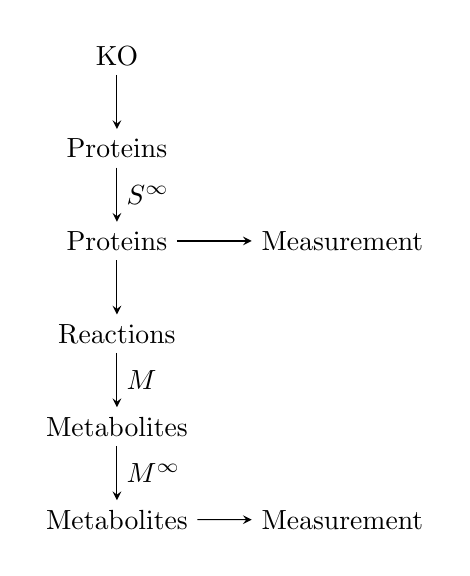
\begin{tikzpicture}
  \matrix (m) [matrix of nodes, row sep = 2em, column sep = 2em]
  {
    KO & \\
    Proteins & \\
    Proteins & Measurement \\
    Reactions & \\
    Metabolites & \\
    Metabolites & Measurement \\
  };
  \path[-stealth]
    (m-1-1) edge (m-2-1)
    (m-2-1) edge node [right] {$S^\infty$} (m-3-1)
    (m-3-1) edge (m-3-2)
      edge (m-4-1)
    (m-4-1) edge node [right] {$M$} (m-5-1)
    (m-5-1) edge node [right] {$M^\infty$} (m-6-1)
    (m-6-1) edge (m-6-2);
\end{tikzpicture}

This framework describes the propagation of changes caused by the KOs through the interaction networks to measured protein and metabolite abundances.\footnote{Where do lipids fit in?}
Here, the matrix $S$ captures regulatory and signaling interactions and the matrix $M$ captures metabolic pathways.

\paragraph{Observation.} If we can assume that there is no pathway for KOs to affect metabolites other than via its effect on proteins, could we treat the problem of predicting changes in metabolites given changes in proteins as a distinct problem from that of predicting changes in proteins given KOs?

\paragraph{Knockout-protein model.}
The matrix $S$ models how proteins interact, more specifically, how the abundance of one protein affects the abundance of another.
This means that entities like protein complexes are only relevant in interactions if they in turn affect the abundances of other proteins (e.g. by affecting regulation).
If we suppose that there is a graph $G$ represents protein interactions, and suppose that in the experiment, there is sufficient time for the effects of knockouts to propagate throughout the graph, $S$ is the transitive closure of $G$.
Moreover, if a change is observed in one protein, the effects of that change must have been observed as well in the model.
If we had access to the true effect matrix $F$, we would have:
\begin{itemize}
 \item $F_{i \cdot} S = F_{i \cdot}$ for each knockout $i$. This is because if a change is observed in a protein, the propagation of that change to other proteins must have also been observed.
 \item If $F_{i j} = F_{i' j} \neq 0$ then $\forall k : S_{j k} \neq 0 \Rightarrow F_{i k} = F_{i' k}$.
 \item $S_{i \cdot} = F_{i \cdot}$.
\end{itemize}
Note that the statements above are not orthogonal.

\paragraph{Protein-metabolite model.}
To easily incorporate known metabolic pathways into the model we first start with the formulation of a pair of binary matrices, $R^\text{in}$ and $R^\text{out}$, where each row corresponds to a reaction and each column a metabolite.
$R^\text{in} - R^\text{out}$ is somewhat similar to a flux matrix, but we don't model stoichiometry here.\footnote{Could we model stoichiometry?}
We also need a matrix that tells us which protein catalyzes which reaction.
Let that be a binary matrix $C$, where each row is a protein and each column is a reaction.
Given these, $C R^\text{in}$ and $C R^\text{out}$ give us matrices where each row is a protein, and each column is a metabolite that potentially accumulates/depletes due to a change in the protein-catalyzed reactions associated.
These changes may in turn propagate through the metabolic network.
To model this propagation we can consider, for a given protein presence/absence vector $\vec p$, $(R^\text{in})^T ( \vec p C ) R^\text{out}$ as the propagation model.
Therefore, given protein presence/absences vector $\vec p$ and protein abundance change vector $\vec{\Delta p}$, the expected change in the metabolite vector $\vec{ \Delta m}$ is bounded as:
\[
 -\vec{\Delta p} C R^\text{out} ( (R^\text{in})^T ( \vec p C ) R^\text{out} )^\infty \leq \vec{ \Delta m} \leq \vec{\Delta p} C R^\text{in} ( (R^\text{in})^T ( \vec p C ) R^\text{out} )^\infty
\]
One implicit assumption is that changes in abundance don't propagate backwards: the accumulation of a product of a reaction does not get potentially propagated to accumulations of the ingredients.

A relaxed version of this model is one that does not take into account the change in available reactions in propagation, this simplifies to
\[
 -\vec{\Delta p} C R^\text{out} \underbrace{( (R^\text{in})^T R^\text{out} )^\infty}_M \leq \vec{ \Delta m} \leq \vec{\Delta p} C R^\text{in} \underbrace{( (R^\text{in})^T R^\text{out} )^\infty}_M
\]
where M is the transitive closure of the metabolic network (for metabolites).

\subsection{Statement as a likelihood}

\paragraph{The protein model.}
The protein model consists of a single, transitively closed, trinary $(-1, 0, 1)$ matrix $G$, but for the optimization formulation, it helps to separate it into two matrices, making up the positive and negative components, $G_+$ and $G_-$ respectively.
We then have the constraints:
\begin{align}
 \left. \begin{aligned}
  G_{+ij} \in \{0,1\} \\
  G_{-ij} \in \{0,1\}
 \end{aligned} \right\} \forall i,j
 &\qquad \text{Domain constraints} \\
 G_{+ij} + G_{-ij} \leq 1 \quad \forall i,j &\qquad \text{Logical consistency constraint} \\
 \left. \begin{aligned}
  G_{+ij} \geq G_{+ik} G_{+kj} \\
  G_{+ij} \geq G_{-ik} G_{-kj} \\
  G_{-ij} \geq G_{-ik} G_{+kj} \\
  G_{-ij} \geq G_{+ik} G_{-kj}
 \end{aligned} \right\} \forall i,j,k
 &\qquad \text{Transitivity constraints}
\end{align}

To derive the likelihood, we view this as a generative model where
\begin{equation}
 D_{ij} = f( G_{ij} )
\end{equation}
For Knockut $i$ and protein $j$, where $f$ is a function from the $\{ -1, 0, 1\}$ space to the space of $D$.
The likelihood part of the optimization is then simply $\sum_{ij} \ell ( i j )$ for pointwise likelihood function $i j$.

\paragraph{Optimizing transitivity.}
The transitive constraints in the na\:ive formulation are quadratic, however, we can replace $G_+, G_-$ with a variable $T$ representing all three-node-paths, defining
\begin{align}
 T_{i+j+k} = G_{+ij} G_{+jk} \quad; i \rightarrow^+ j \rightarrow^+ k \\
 T_{i+j-k} = G_{+ij} G_{-jk} \quad; i \rightarrow^+ j \rightarrow^- k \\
 T_{i-j+k} = G_{-ij} G_{+jk} \quad; i \rightarrow^- j \rightarrow^+ k \\
 T_{i-j-k} = G_{-ij} G_{-jk} \quad; i \rightarrow^- j \rightarrow^- k
\end{align}
where some of these paths are predefined/identical by definition:
\begin{alignat}{3}
 T_{i+i+i} = 1 \qquad & T_{i-i \cdot \cdot} = 0 \qquad & T_{ \cdot \cdot i - i } = 0 \\
 T_{i+i \cdot j} = T_{i \cdot j+j} \qquad &
\end{alignat}
and, as a result, we can represent the transitivity constraints as linear.
However, we need to introduce a constraint for $T$ to accurately maintain its meaning, namely, $T_{i+j+k} = T_{i+j+j} T_{j+j+k}$, which can be rewritten as
\begin{gather}
  T_{i x j \cdot k} \leq T_{i x j+j} \qquad T_{i \cdot j x k} \leq T_{j x k + k} \\
  T_{i x j y k} \geq T_{i x j + j} + T_{j y k + k} - 1
\end{gather}

$T$ is therefore a tensor in $\mathbb R^{n \times 2 \times n \times 2 \times n}$ if we are given $n$ proteins.

\section{Results}

\section{Discussion}

\printbibliography

\end{document}